\title{Benchmarking a Sentiment Analysis Algorithm on Multiple Platforms}


\author{Min Chen}
\affiliation{%
  \institution{Indiana University}
  \streetaddress{School of Informatics, Computing, and Engineering}
  \city{Bloomington}
  \state{IN}
  \postcode{47408}
}
\email{mc43@iu.edu}

\author{Gregor von Laszewski}
\affiliation{%
  \institution{Indiana University}
  \streetaddress{Smith Research Center}
  \city{Bloomington}
  \state{IN}
  \postcode{47408}
}
\email{laszewski@gmail.com}

\author{Bertolt Sobolik}
\affiliation{%
  \institution{Indiana University}
  \streetaddress{School of Informatics, Computing, and Engineering}
  \city{Bloomington}
  \state{IN}
  \postcode{47408}
}
\email{bsobolik@iu.edu}


% The default list of authors is too long for headers}
\renewcommand{\shortauthors}{M. Chen, G. v. Laszewski, B. Sobolik}


\begin{abstract}
A sentiment analysis algorithm is run on several Hadoop
configurations: in pseudo-cluster mode on an Ubuntu 16.04 virtual
machine on a MacBook Pro with and without YARN, in pseudo-cluster mode
in a Docker container on various personal computers and on
Futuresystems Echo, in a cluster created using Docker Compose on
various personal computers and on Futuresystems Echo, and in a cluster
created using Docker Swarm on various Futuresystems Echo. Performance
tests are natural language processing based sentiment analysis on
movie reviews (Polarity 2.0) implemented under MapReduce framework
using Hadoop Streaming. Configurations are described in detail and
steps to recreate them are outlined. In an appendix, steps toward
creating a Hadoop cluster on five networked Raspberry Pi 3 model B
computers in a repeatable and scalable fashion, automating as much of
the setup process as possible are detailed and next steps are
discussed.
\end{abstract}

\keywords{hid-sp18-419, hid-sp18-405, Hadoop, Docker, Futuresystems}


\maketitle

\section{Introduction}
\TODO{Write an introduction.}


\section{Technology Used}

This section describes the technologies that has been utilized
throughout the project. These technologies can be grouped into several
groups: Hadoop, Docker, personal computers, and cloud platforms.

\subsection{Hadoop}

\paragraph{Hadoop}
\paragraph{HDFS}
\paragraph{Hadoop-streaming}
\paragraph{Map-reduce}


\subsection{Docker}
Docker is a technology that allows applications to run in containers
instead of full VMs. It leverages control groups and name space
isolation in the Linux kernel. Containers start up much faster than
VMs and is supported by all the major public cloud
vendors~\cite{Foster:2017:CCS:3158276}. The most current stable
release of Docker Community Edition was used for this project
(18.03.0-ce).
\paragraph{Docker Compose}
\paragraph{Docker Swarm}


\subsection{Cloud Platforms}
\paragraph{Echo}
\paragraph{Google Cloud}


\section{Deployment}\label{s:deployment}
\TODO{Finish Deployment section}
\TODO{Write a section discuss details about deployment of 
hadoop on different platforms, and in different forms}

\section{Data}\label{s:data}

The data used for the project is the Polarity Data 2.0, which is a
dataset of movie reviews, first used by Bo Pang and Lillian
Lee~\cite{hid-sp18-405-sentiment-pang2004asentimental}~\cite{hid-sp18-405-sentiment-pang2002thumbs}.
The dataset includes 1000 positive and 1000 negative processed
reviews, which are labelled with respect to their overall sentiment
polarity.

Each of the review is in a format of text file, and each of the single line in a 
file is corresponding to a sentence. Further, every token (which includes 
single word, punctuation marks, numbers) has been separated by space. For 
example, Figure~\ref{f:data} shows several lines in one of the movie reviews 
with line number on the right, which illustrate the two features mentioned 
above. These features play an important role in the sentiment analysis 
algorithm especially under map-reduce framework, which will be discussed in 
details in Section~\ref{s:algorithm}.
\begin{figure*}[!ht]
	\centering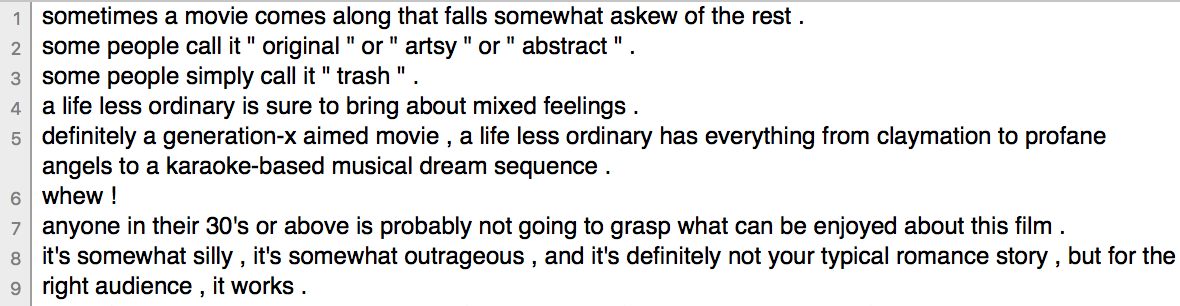
\includegraphics[width=\columnwidth]{images/polarity-data.png}
	\caption{Example Data File}\label{f:data}
\end{figure*}

The data is directly pulled from the 
source~\cite{hid-sp18-405-sentiment-data} and then split into training and 
testing sets according to a ratio of 8:2. The authors also keep the original 
ratio of positive and negative reviews in both the training and testing data 
sets. As a result, there are 1600 reviews (800 positive and 800 negative) in 
the training data set and 400 reviews (200 positive and 200 negative) in the 
testing data set. The splitting process is done by using the random sort 
functionality in bash with a fixed random seed to ensure consistency of 
performance benchmarking on different platforms. 


\section{Algorithm}\label{s:algorithm}

This section introduces the algorithm used to classify the overall sentiment 
of the movie reviews in the benchmarking process. The algorithm is a 
modified version from Pang and 
Lee~\cite{hid-sp18-405-sentiment-pang2004asentimental} and also 
explained in details by Jurafsky and 
Martin~\cite{hid-sp18-405-sentiment-jurafsky2009}. 

\subsection{Baseline algorithm}\label{ss:base}

The baseline algorithm contains the following steps:

\begin{enumerate}
	\item Tokenization
	\item Feature Extraction
	\item Classification
\end{enumerate}

\paragraph{Tokenization}
As mentioned in Section~\ref{s:data}, every token (which includes 
single word, punctuation marks, numbers) has been separated by space in 
the text files. Therefore, we just need to split the text strings with space to 
perform tokenization rather than use sophisticated tokenizers. This saves 
space and running time as well as the complication of loading  python 
packages for hadoop worker nodes in hadoop-streaming. However, in more 
general settings with text data, non-trivial tokenization step needs to be 
performed before other type of text processing.

\paragraph{Feature Extraction}
The main feature that we use is the words contained in the documents, 
however, there are several options mentioned by Jurafsky and 
Martin~\cite{hid-sp18-405-sentiment-jurafsky2009}: 
\begin{enumerate}
	\item All tokens
	\item Removing stoplist words
	\item Removing punctuation tokens
	\item Using only adjectives
	\item Unify tokens with lemmas
	\item Negation treatment
\end{enumerate}
In this project, we applied stoplist words removal, punctuation tokens 
removal and negation treatment. 

Stoplist is the list of words that are considered to be commonly used across 
documents regardless of sentiments thus adding little value in classification 
tasks. We removed stoplist words according to the english stopwords 
module from the python package: NLTK 
corpus~\cite{hid-sp18-405-sentiment-stopworddoc}. Punctuation removal is 
done by using python string 
module~\cite{hid-sp18-405-sentiment-punctuationdoc} supplemented by 
self-defined regular expression. We applied a basic negation treatment by 
adding a NOT\_ prefix to every token that follows a negation word and not 
separated by any punctuation tokens. For example: I really do not like the 
movie becomes: I really do not Not\_like Not\_the Not\_movie. This method is 
used by Das and Chen~\cite{hid-sp18-405-sentiment-das2001yahoo} as well 
as Pang, Lee, and 
Vaithyanathan~\cite{hid-sp18-405-sentiment-pang2002thumbs}. 

We did not apply the option of using adjectives only due to the result 
provided by Pang and his 
colleges~\cite{hid-sp18-405-sentiment-pang2004asentimental} that  
adjectives only does not provide a better results than including all words. In 
fact, the accuracy dropped by on average 2\% in the testing phase when we 
implemented the algorithm. We also did not apply lemmatization for all the 
tokens. Although lemmatization would increase the accuracy by around 2\% 
in one of the authors previous studies, it requires ontologies such as 
wordnet and including the wordnet corpus with lemmatizer is adding much 
complication to the hadoop-streaming. We tried to follow the instructions 
online~\cite{hid-sp18-405-hadoopstreaming-nltk}~\cite{hid-sp18-405-hadoopstreaming-corpus}
 to pass python package (NLTk) and corpus (wordnet) as zipped files from 
name nodes to data nodes in mapreduce tasks but the package can be 
passed but not loaded and corpus cannot be passed. This issue could be 
studied and solved in future projects. 

Pang, Lee, and 
Vaithyanathan~\cite{hid-sp18-405-sentiment-pang2002thumbs}, also 
considered different set of 
features such as bigrams, combination (back up) of bigrams and unigrams, 
top-unigrams etc. For simplicity, we chose to only use unigram models i.e. 
single tokens. 

\paragraph{Classifier}
We  used Naive Bayes as the classifier. The formulation is given as:
\begin{equation}\label{eq:nb}
c_{NB}=\text{argmax}_{c_j \in C} P(c_j) \prod_{i \in positions} P(w_i|c_j)
\end{equation}

where in this case, $j \in \{positive, negative\}$, also for this movie review 
dataset, we know the prior probabilities: 
$P(c_{positive})=P(c_{negative})=0.5$

\paragraph{Smoothing}
To avoid the problem that the probability of some token in the 
training/testing document is zero. We use the add-one smoothing or Laplace 
smoothing in this case:
\begin{equation}\label{eq:sm}
P(w|c) = \frac{count(w,c) + 1}{count(c) + |V|}
\end{equation}

Figure~\ref{f:algo} is the algorithm we implemented summarized by Jurafsky 
and Martin:
\begin{figure}[!ht]
		\centering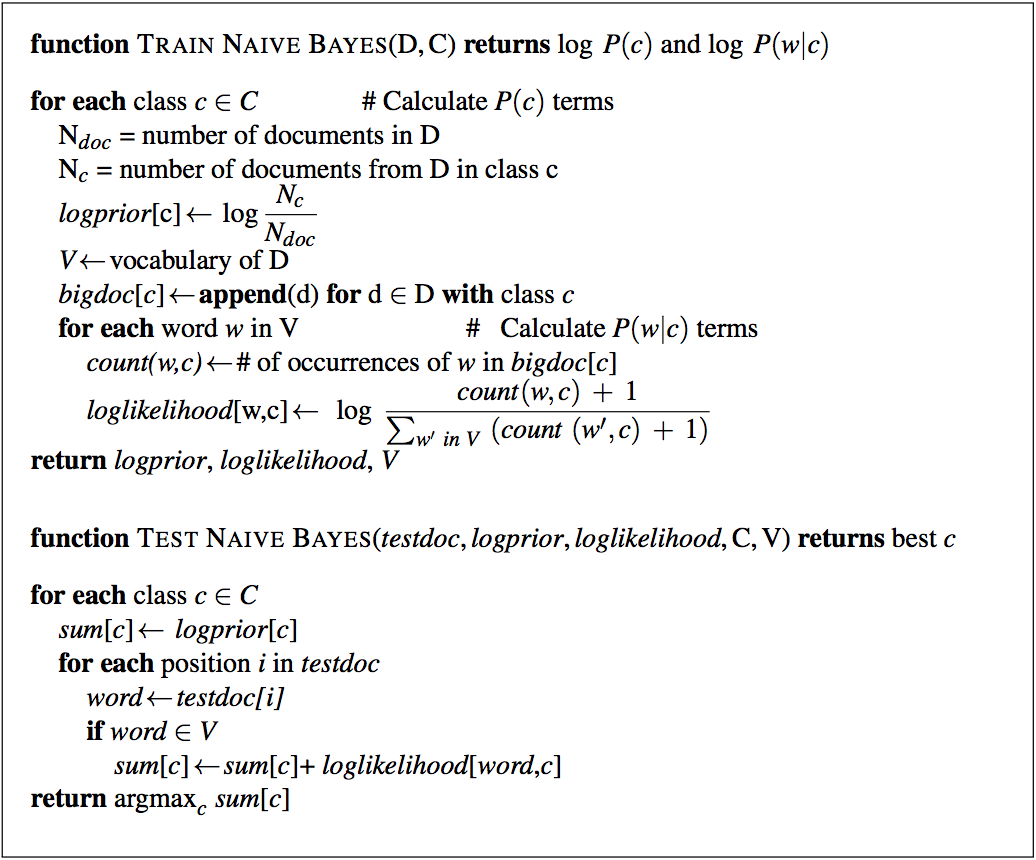
\includegraphics[width=\columnwidth]{images/algorithm.png}
		\caption{Naive Bayes for Sentiment 
		Analysis~\cite{hid-sp18-405-sentiment-jurafsky2009}}\label{f:algo}
\end{figure}

\subsection{Implementation using MapReduce}

As illustrated in Equation~\ref{eq:nb}, Equation~\ref{eq:sm}, and 
Figure\ref{f:algo}, the Naive Bayes classification algorithm is based on 
comparing posterior probability. The likelihood of each single valid token can 
be calculated by aggregating the count of this token among the training 
documents for the two classes positive and negative. The the likelihood of a 
testing document is an aggregation of the likelihood of each valid token 
within that document. Therefore, both training and testing process can be 
implemented in a MapReduce framework to facilitate the process of counting 
tokens and aggregation. 

There are two MapReduce jobs in the training process, one for training on 
positive-labelled documents and the other for negative-labelled documents. 
$count(w,c)$ in Equation~\ref{eq:sm} shows the necessity to count the 
tokens according to the classes, which are positive and negative in this task. 
During the training on positive-labelled documents, the TrainingMapper 
python code will read in each positive movie reviews in the training set 
through standard input, filter valid tokens (removing stoplist words, 
punctuation, adding negation, see Subsection\ref{ss:base}) and print to the 
standard output. TrainingReducer python code will take these standard 
output performing aggregation by tokens. The result is a dictionary-like text 
file containing number of occurrence for each valid token in the positive 
training set. The negative training documents will be processed in a similar 
way. 

 In the testing process, each testing document is analyzed separately. The 
 TestingMapper will read in the one document, perform the same filter to 
 keep valid tokens and print to standard output. The testingReducer will read 
 in both this standard output and the two results files from the training 
 process, calculating the likelihood of each valid token in this document 
 according to the smoothing formula given by Equation~\ref{eq:sm} before 
 getting posterior probability through aggregation according to 
 Equation~\ref{eq:nb}. Then for each document, there will be two posterior 
 probabilities, positive and negative. The document will be assigned to the 
 one with higher probability. The final output will be a text file and each line is 
 the testing document name with its classification label. In the actual 
 implementation, we performed the testing process using two MapReduce 
 jobs, one for the testing data that are actually positive, the other for the 
 testing data that are actually negative. This is essentially the same as 
 performing testing process on each document blindly and then verify the 
 results. However, it is easier to calculate the accuracy of the algorithm. 
 
 In summary, we used python codes to implement two mappers 
 (TrainingMapper and TestingMapper) and two reducers (TrainingReducer 
 and Testingreducer) to perform 4 MapReduce jobs for the training and 
 testing processes. For the fixed random seed mentioned in 
 Section\ref{s:data}, we achieved the following results: out of the 200 
 positive testing data, 162 are correctly labelled; out of the 200 negative 
 testing data, 168 are correctly labelled. Therefore, the
 overall accuracy of the algorithm is 82.5\%. This is acceptable 
 compared to the result achieved by Pang, Lee, and Vaithyanatha, which is 
 illustrated in Figure\ref{f:pang-result}. 
% 
%\begin{figure}[!ht]
%	\centering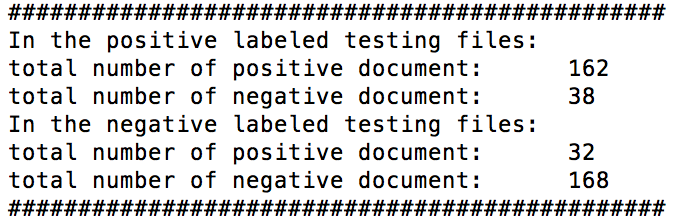
\includegraphics[width=\columnwidth]{images/algoresult.png}
%	\caption{Results of the Algorithm}
%	\label{f:algoresult}
%\end{figure}

\begin{figure}[!ht]
	\centering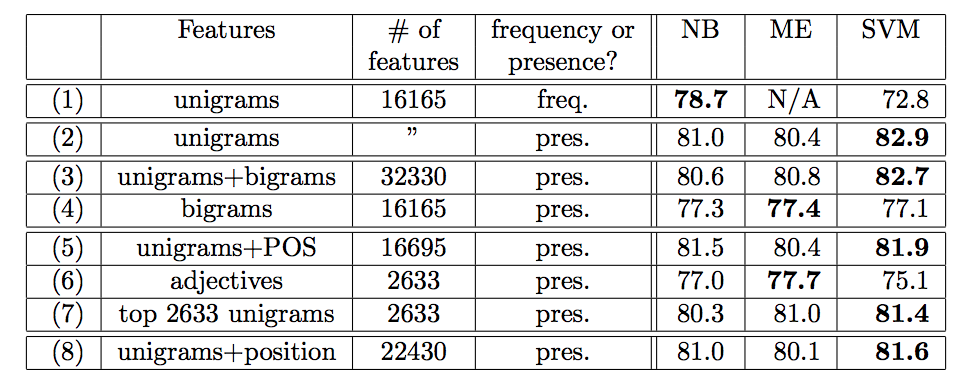
\includegraphics[width=\columnwidth]{images/pang-result.png}
        \caption{Results
	from Pang, Lee, and Vaithyanatha
	(2002)~\cite{hid-sp18-405-sentiment-pang2002thumbs}}\label{f:pang-result}
\end{figure}


\section{Hadoop Deployment}\label{s:hadoopdep}

\subsection{Pseudo Distributed}
\paragraph{Direct Installation}
\paragraph{Dockerized Installation}

\subsection{Fully Distributed using docker compose}


\subsection{Fully Distributed using docker swarm}


\section{Benchmarking Process}
\TODO{Describe machines and platform used, data points collection}


\section{Results}
\TODO{Add results.}

\begin{table}[hbt]
\centering
\caption{Benchmarking results}\label{t:results-table}
\begin{tabular}{llll}
Platform    & Docker & Deployment time & MapReduce Time \\
Pi 5 nodes  & Yes    & TBD             & TBD            \\
Pi 5 nodes  & No     & TBD             & TBD            \\
Echo        & Yes    & TBD             & TBD            \\
Echo        & No     & TBD             & TBD            \\
\end{tabular}
\end{table}



\section{Conclusion}

\TODO{Put here an conclusion. Conclusion and abstracts must not have any
citations in the section.}

\section{Appendix: Hadoop Cluster on Raspberry Pi}
This section describes steps taken toward the goal of creating a
Hadoop cluster using 5 Raspberry Pi 3 Model B computers in a
repeatable, scalable way. Successes and challenges are described and
recommended next steps are outlined.

\subsection{Hardware}

The hardware used for the Raspberry Pi cluster consists of:

\begin{itemize}
\item Five Raspberry Pi 3 Model B computers 
\item One Waveshare 4in HDMI LCD touchscreen
\item One Netgear model GS308 8-Port Gigabit ethernet switch
\item One Anker PowerPort 6 USB power supply
\item One Powtech 125V AC 15A 1875w adaptor with switch
\item Five 1-foot ethernet cables
\item Five 32 GB microSDHC UHS-I cards
\item Six 6in USB 2.0 A-Male to Micro B cables
\item 24 20mm by 5mm Hex Hexagonal Threaded Spacer Supports
\end{itemize}

A pinout diagram of the Pi 3B is shown in Figure~\ref{f:pinout-diagram}.

\begin{figure*}[!ht]
  \centering\includegraphics[width=\columnwidth]{images/raspberry_pi_circuit_note_fig2.png} \caption{Pinout
  diagram of Raspberry Pi 3B~\cite{hid-sp18-419-pi-pinout}. Note: the
  Pi used for this project has a Broadcom BCM2837, not the Broadcom
  BMC2835 shown in this figure.}\label{f:pinout-digram}
\end{figure*}

\subsection{Building a Pi Cluster}
\TODO{Finish building descrition. Depending on how elaborate this
is, it could be folded into the deployment section instead of being in
it's own section.}  Physical assmebly of the cluster is fairly
simple. First, aluminium and copper heat syncs need to be attached to
each Pi. The two aluminium heat syncs are attached to the Broadcom
chip and the SMSC ethernet controller located on the top of the
Pi. The blades of the heat syncs are parallel to the longer side of
the Pi as shown in Figure~\ref{f:heat-sync-top}.

\begin{figure*}[!ht]
  \centering\includegraphics[width=\columnwidth]{images/heat-sync-top.jpg} \caption{Top
  view of a Raspberry Pi 3B with heat syncs
  attached.}\label{f:heat-sync-top}
\end{figure*}

The flat copper heat sync is attached to the Elpida RAM on the bottom
of the Pi as shown in Figure~\ref{f:heat-sync-bottom}.

\begin{figure*}[!ht]
  \centering\includegraphics[width=\columnwidth]{images/heat-sync-bottom.jpg} \caption{Bottom
  view of a Raspberry Pi 3B with heat sync
  attached.}\label{f:heat-sync-bottom}
\end{figure*}

After attaching the heat syncs, threaded hexagonal spacer supports are
used to connect the Pis together. A fully-assembled 5-node Pi cluster
is shown in Figure~\ref{f:cluster-no-wires}.

\begin{figure*}[!ht]
  \centering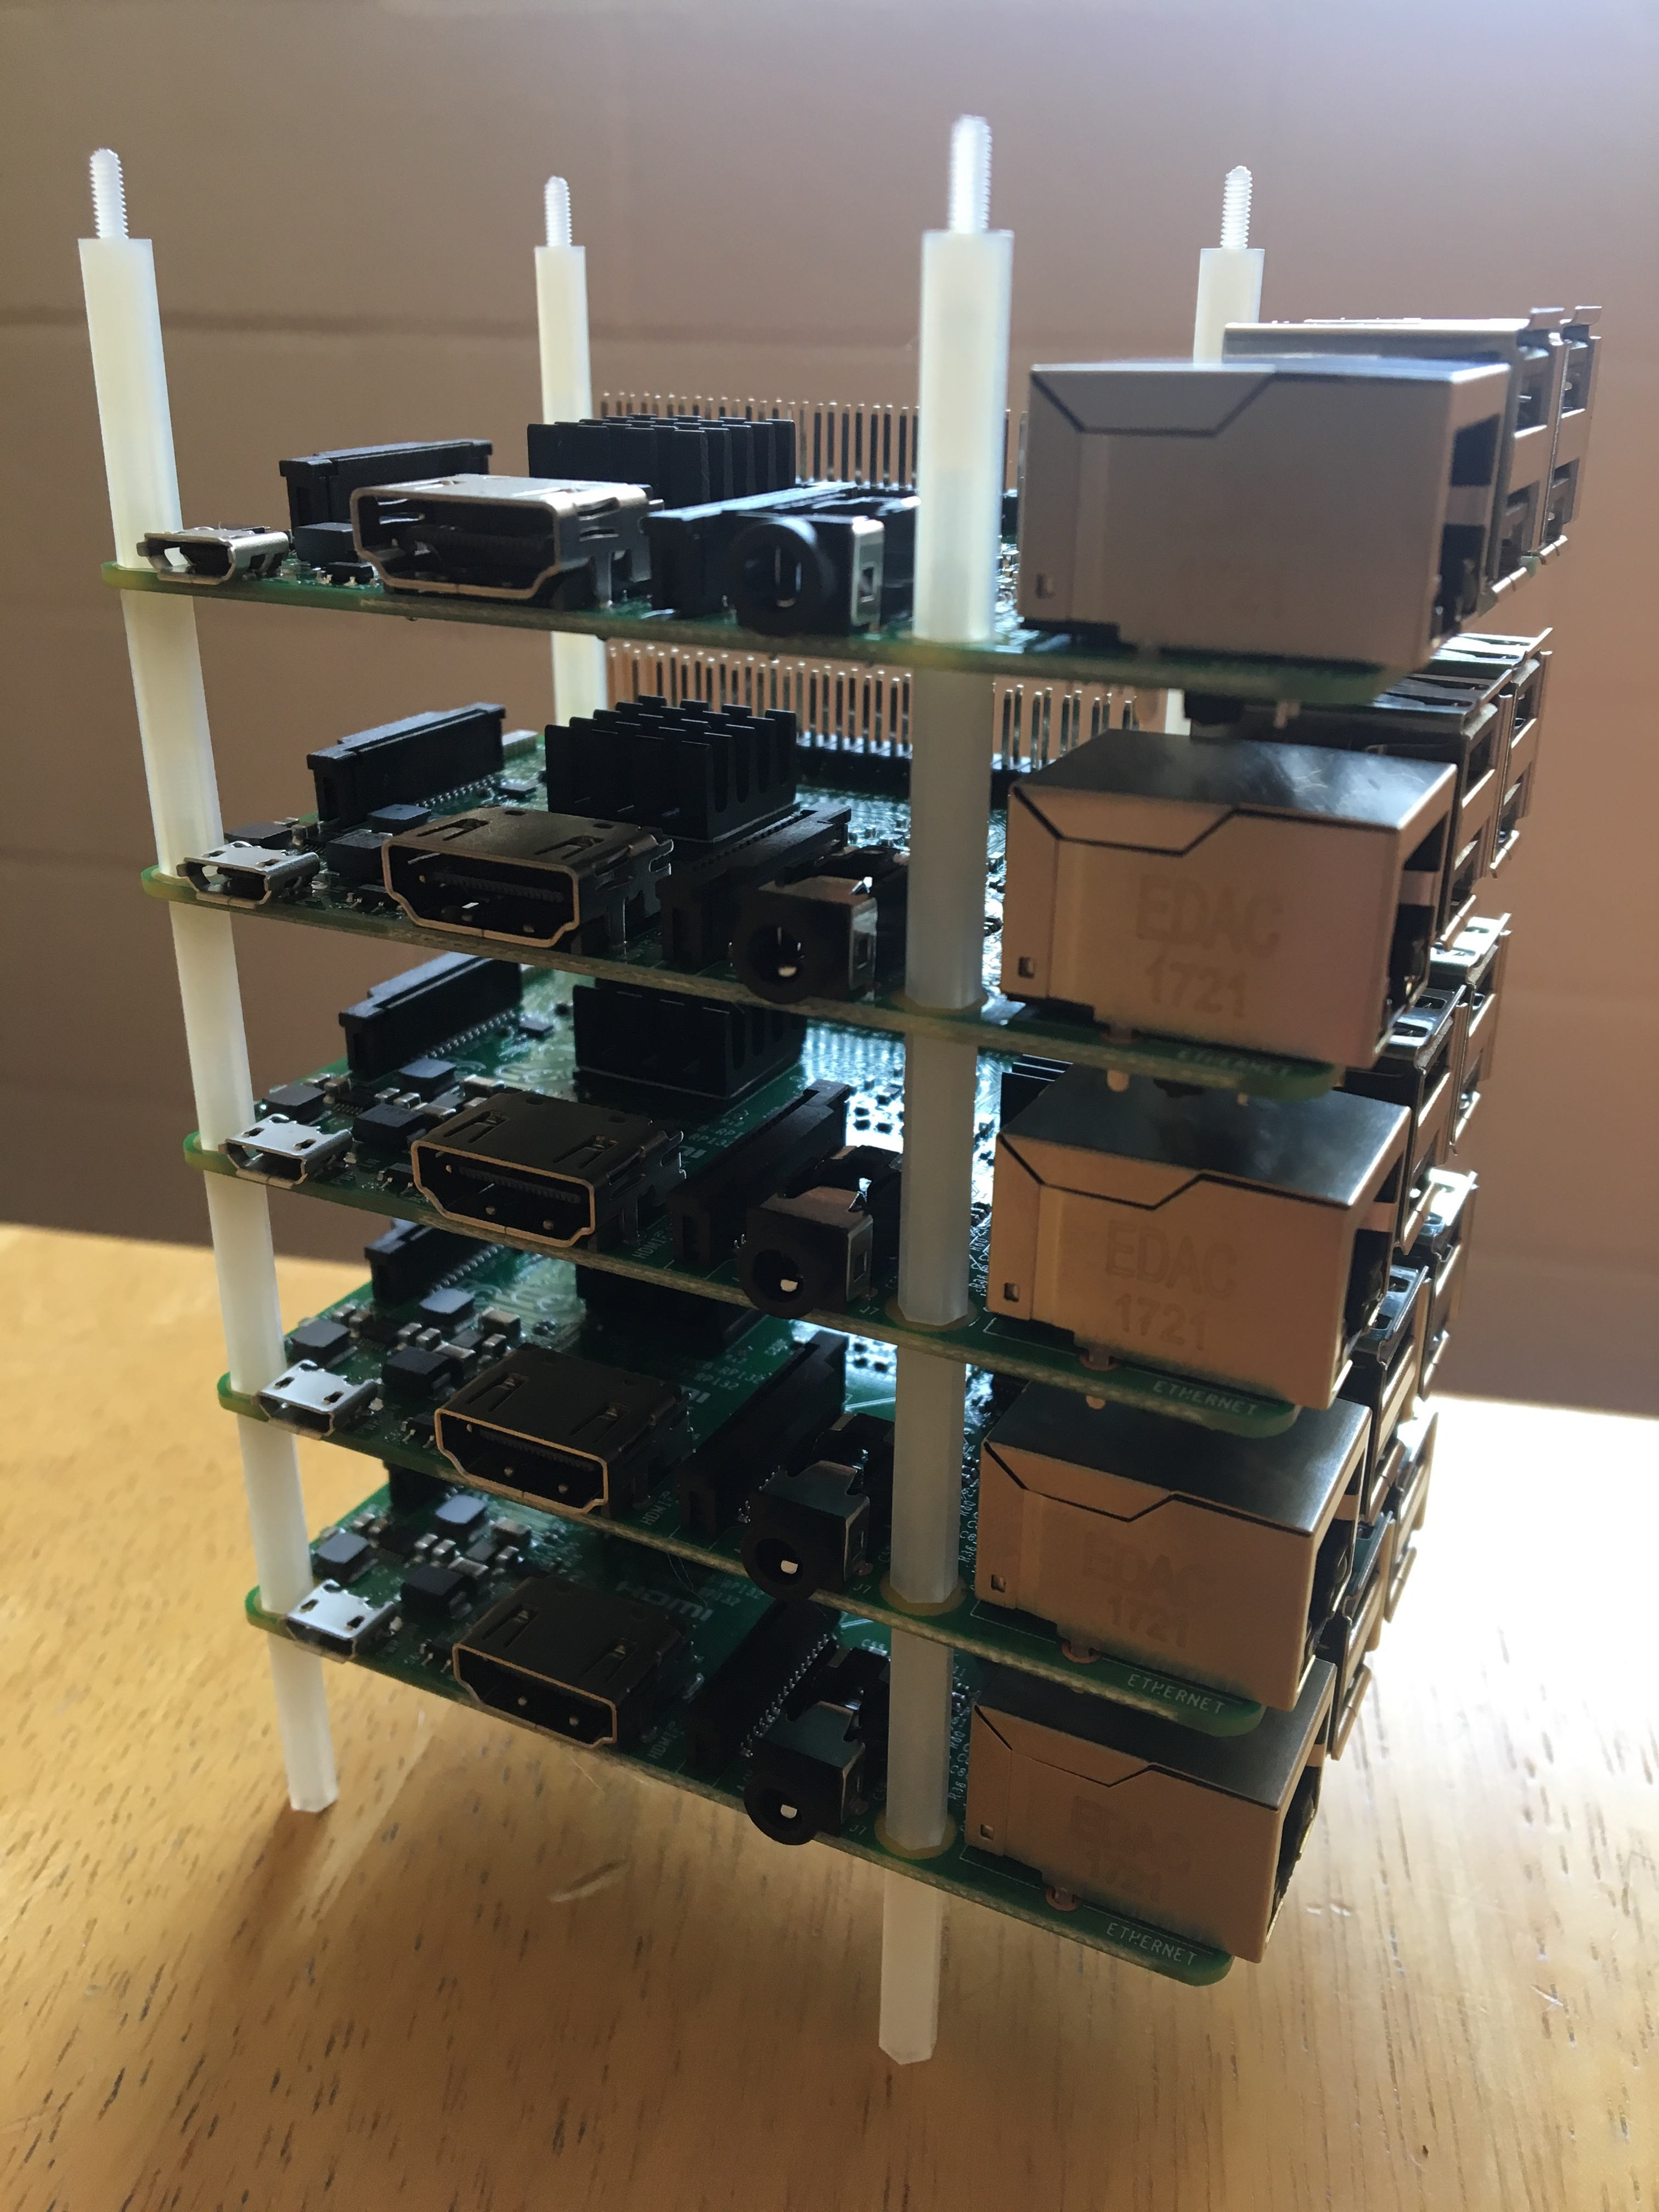
\includegraphics[width=\columnwidth]{images/pi-cluster-no-wires.jpg}
  \caption{5-node Pi cluster before wiring.}\label{f:cluster-no-wires}
\end{figure*}

Each node of the cluster is then attached to the switch using the
ethernet cables.

\subsection{Configuring the Pi Cluster}
To configure the Raspberry Pis, first SD cards were burned using a
script that takes start and end machine id numbers as an input. The
option to perform DHCP setup can be enabled with a flag. If DHCP is
not used, the script assigns static IPs to each machine.

\begin{acks}

  The authors would like to thank Dr.~Gregor~von~Laszewski for his
  support and suggestions to write this paper.

\end{acks}

\bibliographystyle{ACM-Reference-Format}
\bibliography{report}
